\chapter{\foreignlanguage{english}{UML} Διαγράμματα}

Στην παρούσα ενότητα παρουσιάζονται δύο βασικά διαγράμματα \foreignlanguage{english}{UML} για την τεκμηρίωση της λειτουργικότητας και της αρχιτεκτονικής της εφαρμογής.

Το \foreignlanguage{english}{\textbf{Class Diagram}} απεικονίζει τις κύριες κλάσεις και τις μεταξύ τους σχέσεις, με έμφαση στη ροή δεδομένων και τις κύριες μεθόδους.

\begin{figure}[h]
    \centering
    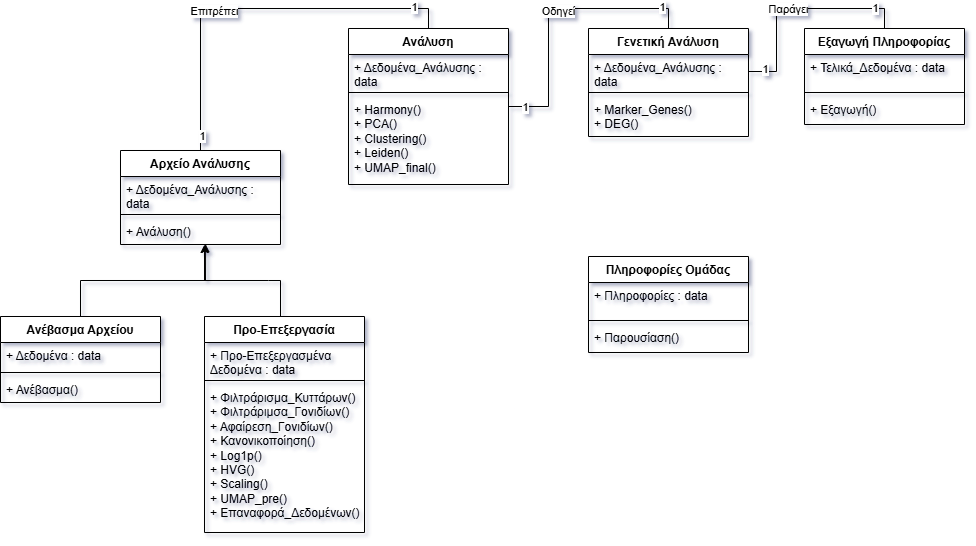
\includegraphics[width=0.95\textwidth]{images/Class_Diagram.png}
    \caption{\foreignlanguage{english}{UML Class Diagram} της εφαρμογής}
\end{figure}

\newpage

Το \foreignlanguage{english}{\textbf{Use Case Diagram}} περιγράφει τις ενέργειες που εκτελεί ο χρήστης μέσα στην εφαρμογή, καθώς και τις σχέσεις μεταξύ των διεργασιών \foreignlanguage{english}{(use cases)} που υλοποιούνται μέσω των διαφορετικών \foreignlanguage{english}{tabs}.

\begin{figure}[h]
    \centering
    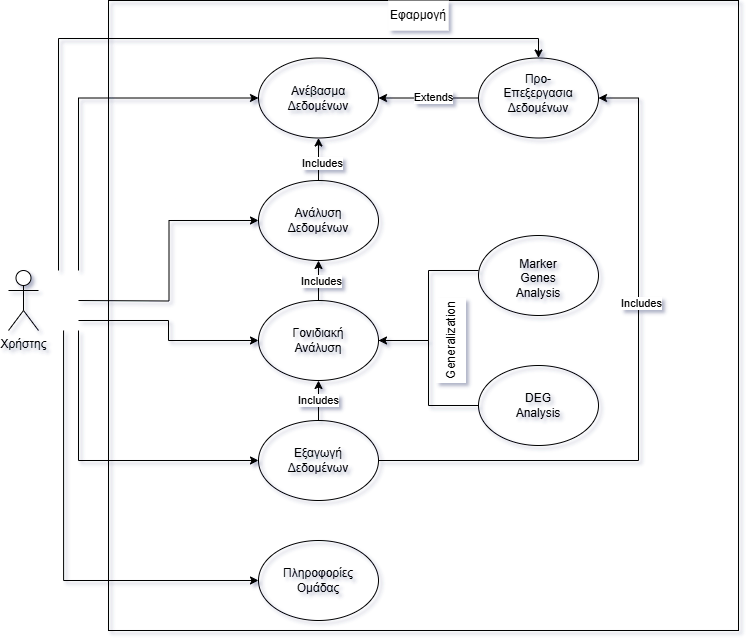
\includegraphics[width=0.9\textwidth]{images/Use_Case_Diagram.png}
    \caption{\foreignlanguage{english}{Use Case Diagram} της εφαρμογής}
\end{figure}
